% This is "sig-alternate.tex" V1.9 April 2009
% This file should be compiled with V2.4 of "sig-alternate.cls" April 2009
%
% This example file demonstrates the use of the 'sig-alternate.cls'
% V2.4 LaTeX2e document class file. It is for those submitting
% articles to ACM Conference Proceedings WHO DO NOT WISH TO
% STRICTLY ADHERE TO THE SIGS (PUBS-BOARD-ENDORSED) STYLE.
% The 'sig-alternate.cls' file will produce a similar-looking,
% albeit, 'tighter' paper resulting in, invariably, fewer pages.
%
% ----------------------------------------------------------------------------------------------------------------
% This .tex file (and associated .cls V2.4) produces:
%       1) The Permission Statement
%       2) The Conference (location) Info information
%       3) The Copyright Line with ACM data
%       4) NO page numbers
%
% as against the acm_proc_article-sp.cls file which
% DOES NOT produce 1) thru' 3) above.
%
% Using 'sig-alternate.cls' you have control, however, from within
% the source .tex file, over both the CopyrightYear
% (defaulted to 200X) and the ACM Copyright Data
% (defaulted to X-XXXXX-XX-X/XX/XX).
% e.g.
% \CopyrightYear{2007} will cause 2007 to appear in the copyright line.
% \crdata{0-12345-67-8/90/12} will cause 0-12345-67-8/90/12 to appear in the copyright line.
%
% ---------------------------------------------------------------------------------------------------------------
% This .tex source is an example which *does* use
% the .bib file (from which the .bbl file % is produced).
% REMEMBER HOWEVER: After having produced the .bbl file,
% and prior to final submission, you *NEED* to 'insert'
% your .bbl file into your source .tex file so as to provide
% ONE 'self-contained' source file.
%
% ================= IF YOU HAVE QUESTIONS =======================
% Questions regarding the SIGS styles, SIGS policies and
% procedures, Conferences etc. should be sent to
% Adrienne Griscti (griscti@acm.org)
%
% Technical questions _only_ to
% Gerald Murray (murray@hq.acm.org)
% ===============================================================
%
% For tracking purposes - this is V1.9 - April 2009

\documentclass[letter]{sig-alternate}
\special{papersize=8.5in,11in}

\makeatletter
\newif\if@restonecol

\let\algorithm\relax
\let\endalgorithm\relax
\usepackage[tight,footnotesize]{subfigure}
\usepackage {paralist}
\usepackage{comment}
\usepackage{array}
\usepackage{amsmath}
%\usepackage{amsthm}
\usepackage{graphicx}
\usepackage{amssymb}
\usepackage{url}
\usepackage[ruled]{algorithm2e}
\makeatother
\makeatletter
\providecommand{\tabularnewline}{\\}
\newtheorem{clm}{Claim}
\newtheorem{mydef}{Definition}



\begin{document}
%
% --- Author Metadata here ---
%\conferenceinfo{WOODSTOCK}{'97 El Paso, Texas USA}
%\CopyrightYear{2007} % Allows default copyright year (20XX) to be over-ridden - IF NEED BE.
%\crdata{0-12345-67-8/90/01}  % Allows default copyright data (0-89791-88-6/97/05) to be over-ridden - IF NEED BE.
% --- End of Author Metadata ---

\title{On Real-Time STM Concurrency Control for Embedded Software with Improved Schedulability}

\begin{comment}
\numberofauthors{2}

\author{
\alignauthor
Mohammed Elshambakey\\
       \affaddr{ECE Dept., Virginia Tech}\\
       \affaddr{Blacksburg, VA 24060, USA}\\
       \email{shambake@vt.edu}
\alignauthor
Binoy Ravindran\\
       \affaddr{ECE Dept., Virginia Tech}\\
       \affaddr{Blacksburg, VA 24060, USA}\\
       \email{binoy@vt.edu}
}
\end{comment}

\maketitle
\begin{abstract}
We consider software transactional memory (STM) concurrency control for embedded multicore real-time software, and present a novel contention manager for resolving transactional conflicts, called PNF. We upper bound transactional retries and task response times, and show when PNF has better schedulability than previous contention managers and lock-free synchronization. Our implementation in the Rochester STM framework/real-time Linux reveals that PNF yields shorter or comparable retry costs than competitors.
\end{abstract}

\category{C.3}{Special-Purpose and Application-based Systems}{Real-time and embedded systems}
%\category{D.4.1}{Operating Systems}{Process Management}--{synchronization}
\category{D.4.7}{Operating Systems}{Organization and Design}--{real-time systems and embedded systems}
\terms{Design, Experimentation, Measurement}
\keywords{Software transactional memory (STM), real-time}

\section{Introduction}

%Embedded systems sense physical processes and control their behavior, typically through feedback loops. Since physical processes are concurrent, computations that control them must also be concurrent, enabling them to process multiple streams of sensor input and control multiple actuators, all concurrently. Often, such computations need to concurrently read/write shared data objects. They must also process sensor input and react, while satisfying time constraints. 

The de facto standard for concurrent programming is the threads abstraction, and the 
de facto synchronization abstraction is locks. Lock-based concurrency control has significant programmability, scalability, and composability challenges~\cite{Herlihy:2006:AMP:1146381.1146382}. Software transactional memory (STM) is an alternative synchronization model for shared memory data objects that promises to alleviate these difficulties. With STM, code that read/write shared objects is organized as transactions, which execute speculatively, while logging changes made to objects. Two transactions conflict if they access the same object and one access is a write. When that happens, a contention manager (CM)~\cite{Guerraoui:2005:TTT:1073814.1073863} resolves the conflict by aborting one and allowing the other to commit, yielding (the illusion of) atomicity. Aborted transactions are re-started, after rolling back the changes. In addition to a simple programming model, STM provides performance comparable to locking and lock-free approaches (see an example STM system's performance in~\cite{Saha:2006:MHP:1122971.1123001}), and is composable~\cite{Harris:2005:CMT:1065944.1065952}.  
%TM has been proposed in hardware, called HTM, and in software, called STM, with the usual tradeoffs: HTM has lesser overhead, but needs transactional support in hardware; STM is available on any hardware.


Given STM's programmability, scalability, and composability advantages, it is a compelling concurrency control technique also for multicore embedded real-time software. However, this requires  bounding transactional  retries, as real-time threads, which subsume transactions, must satisfy time constraints.  Retry bounds under STM are dependent on the CM policy at hand (analogous to the way thread response time bounds are OS scheduler-dependent). 
%Thus, real-time CM is logical.


Past real-time CM research has proposed resolving transactional contention using dynamic and fixed priorities of parent threads, resulting in EDF-based CM (ECM) and RMS-based CM (RCM), respectively~\cite{6045438,
%fahmy2009bounding,fahmy2009response,
stmconcurrencycontrol:emsoft11,lcmdac2012}.
In particular,~\cite{stmconcurrencycontrol:emsoft11} shows that ECM and RCM achieve higher schedulability -- i.e., greater number of task sets meeting their time constraints -- than lock-free synchronization only under some ranges for the maximum atomic section length. That range is significantly expanded with the LCM contention manager in~\cite{lcmdac2012}, increasing the coverage of STM's timeliness superiority. However, these works restrict to \textit{one} object access per transaction, which is a major  limitation (Section~\ref{probelm description}). 
%(though not uncommon for embedded systems).
%~\cite{lcmdac2012} presents the LCM CM, which resolves conflicts using the priorities of transactions as well as the relative lengths of interfering and interfered transactions. 
%A higher priority transaction $s_i^k(\theta)$ cannot abort a lower priority transaction $s_j^l(\theta)$ if $s_j^l(\theta)$ has already consumed $\alpha$ percentage of its execution time. 

To allow multiple objects per transaction, we design a novel contention manager called PNF  (Section~\ref{PNF}), which can be used with global EDF (G-EDF) and global RMA (G-RMA) multicore real-time schedulers~\cite{Davis:2011:SHR:1978802.1978814}. 
We upper bound transactional retry costs and task response times (Section~\ref{rc pnf sec}), and formally compare PNF's schedulability with ECM, RCM, LCM, and lock-free synchronization (Section~\ref{sec:pnf-sched-comparison}). 
We show that PNF achieves better schedulability than lock-free synchronization for larger 
atomic section length range than ECM and RCM. 
%bigger value of $s_{max}/r_{max}$ than ECM and RCM.
Our implementation reveals that PNF yields shorter or comparable retry costs than competitors (Section~\ref{exp_eval}).

PNF's superior timeliness properties thus allow embedded real-time programmers to reap STM's significant programmability and composability advantages for a broader range of multicore embedded real-time software than what was previously possible -- paper's contribution. 

Our complete implementation is publicly available at a website, but is withheld due to conference anonymity rules. 
%Our compete implementation is publicly available at a website, which is withheld here to respect conference anonymity rules. 

\begin{comment}
\section{Related Work}
\label{sec:past}

Transactional-like concurrency control without using locks, for real-time systems, has been previously studied in the context of non-blocking data structures (e.g.,~\cite{anderson95realtime}). Despite their numerous advantages over locks 
(e.g., deadlock-freedom), their programmability has remained a challenge.  
%Past studies show that they are best suited for simple data structures where their retry cost is competitive to the cost of lock-based synchronization~\cite{bc+08}.  
In contrast, STM has better programmability, and composes~\cite{Herlihy:2006:AMP:1146381.1146382}.  
%and is often the only viable lock-free solution for complex data structures~\cite{6045438} and nested critical sections~\cite{Saha:2006:MHP:1122971.1123001}.

STM concurrency control for real-time systems has been previously studied. \cite{manson2006preemptible} proposes a restricted version of STM for uniprocessors. Uniprocessors do not need contention management. \cite{fahmy2009bounding} bounds response times in distributed multiprocessor systems with STM synchronization. They limit to small atomic regions with fixed size, and limit transaction execution to span at most two quanta. In contrast, we allow arbitrary-size transaction lengths. \cite{sarni2009real} presents real-time scheduling of transactions and serializes transactions based on deadlines, but does not bound retries and response times. In contrast, we establish such bounds.


\cite{schoeberl2010rttm} proposes real-time HTM, but does not describe how transactional conflicts are resolved. Besides, the retry bound assumes that the worst case conflict between atomic sections occurs when the sections are simultaneously released. However, we show that this is not the worst case, and develop retry bounds based on much worse conditions.


\cite{6045438} upper bounds retries and response times for  ECM with G-EDF. Similar to~\cite{schoeberl2010rttm},~\cite{6045438} also assumes that the worst case conflict occurs when atomic sections are released simultaneously. The ideas in~\cite{6045438} are extended in~\cite{barrosmanaging}, which presents three real time CMs, but no retry bounds or schedulability analysis techniques are presented. 

\cite{stmconcurrencycontrol:emsoft11} presents ECM and RCM, and upper bounds retries and response times under them. However,~\cite{stmconcurrencycontrol:emsoft11} restricts transactions to access only one object. \cite{lcmdac2012} presents LCM, and upper bounds retries and response times. Similar to~\cite{stmconcurrencycontrol:emsoft11},~\cite{lcmdac2012} also restricts transactions to access only one object.

Our work builds upon~\cite{stmconcurrencycontrol:emsoft11, lcmdac2012}, allows multiple objects per transaction, and bounds transactional retries and task response times with improved schedulability. 
\end{comment}

\section{Preliminaries}
\label{sec:model}

We consider a multiprocessor system with $m$ identical processors and $n$ sporadic tasks $\tau_1, 
%\tau_2,
\ldots, \tau_n$. The $k^{th}$ instance (or job) of a task $\tau_i$ is denoted $\tau_i^k$. Each task $\tau_i$ is specified by its worst case execution time (WCET) $c_i$, its minimum period $T_i$ between any two consecutive instances, and its relative deadline $D_i$, where $D_i=T_i$. Job $\tau_i^j$ is released at time $r_i^j$ and must finish no later than its absolute deadline $d_i^j=r_i^j+D_i$. Under a fixed priority scheduler (e.g., G-RMA), $p_i$ determines $\tau_i$'s (fixed) priority and it is constant for all instances of $\tau_i$. Under a dynamic priority scheduler (e.g., G-EDF), $\tau_i^j$'s priority, $p_i^j$, differs across instances. 
A task $\tau_j$ may interfere with task $\tau_i$ for a number of times during an interval $L$, and this number is denoted as $G_{ij}(L)$. 

\textit{Shared objects.} A task may need to access (i.e., read, write) shared memory objects while it is executing any of its atomic sections, which are synchronized using STM. 
(We use the terms ``atomic section" and ``transaction" interchangeably.)
The set of atomic sections of task $\tau_i$ is denoted $s_i$. $s_i^k$ is the $k^{th}$ atomic section of $\tau_i$. 
Atomic section $s_i^k$ may access multiple objects.
Each object, $\theta$, can be accessed by multiple tasks. The set of distinct objects accessed by $\tau_i$ is $\theta_i$.
The set of atomic sections used by $\tau_i$ to access $\theta$ is $s_i(\theta)$, and the sum of the lengths of those atomic sections is $len(s_i(\theta))$. $s_i^k(\theta)$ is the $k^{th}$ atomic section of $\tau_i$ that accesses $\theta$. $s_i^k(\theta)$  executes for a duration $len(s_i^k(\theta))$.
%
Atomic sections are non-nested, and the set of tasks sharing objects with $\tau_i$ is denoted as $\gamma_i$. 
The maximum-length atomic section in $\tau_i$ that accesses $\theta$ is denoted $s_{i_{max}} (\theta)$, while the maximum one among all tasks is $s_{max} (\theta)$, and the maximum one among tasks with priorities lower than that of $\tau_i$ is $s_{max}^i (\theta)$.

\textit{STM retry cost.} If two or more atomic sections conflict, the CM will commit one section and abort and retry the others, increasing the time to execute the aborted sections. The increased time that an atomic section $s_i^p (\theta)$ will take to execute due to conflict with another section $s_j^k (\theta)$, is denoted $W_{i}^{p}(s_{j}^{k}(\theta))$. If an atomic section, $s_i^p$, is executing, and another atomic section $s_j^k$ tries to access a shared object with $s_i^p$, then $s_j^k$ is said to ``interfere" or ``conflict" with $s_i^p$. The job of $s_j^k$ is called the ``interfering job", while the job of $s_i^p$ is called the ``interfered job". 
%
The total time that a task $\tau_i$'s atomic sections have to retry over $T_i$ is denoted $RC(T_i)$.
The additional amount of time $\tau_j$ provides when interfering with $\tau_i$ during $L$, without considering retrial due to atomic sections, is denoted $W_{ij}(L)$.


\section{Limitations of ECM, RCM, and LCM}\label{probelm description}

%\begin{comment}
ECM and RCM~\cite{stmconcurrencycontrol:emsoft11} use dynamic and fixed priorities, respectively, to resolve conflicts. ECM uses G-EDF, and allows the transaction whose job has the earliest absolute deadline to commit first~\cite{6045438}. RCM uses G-RMA, and commits the transaction whose job has the shortest period.

Retry cost under ECM is bounded in~\cite{stmconcurrencycontrol:emsoft11} as follows:

Claim 1 (from~\cite{stmconcurrencycontrol:emsoft11}): Under ECM, a task $\tau_i$'s maximum retry cost during $T_i$ is upper bounded by:
\begin{eqnarray}
RC\left(T_{i}\right) & \le & \sum_{\theta\in\theta_{i}}\Bigg(\Big(\sum_{\tau_{j}\in\gamma_i(\theta)}\Big(\left\lceil\frac{T_{i}}{T_{j}}\right\rceil\sum_{\forall s_{j}^{l}(\theta)}len\big(s_{j}^{l}(\theta)\nonumber \\
 & + & s_{max}(\theta)\big)\Big)\Big)-s_{max}(\theta)+s_{i_{max}}(\theta)\Bigg)\label{eq3}\end{eqnarray}

Retry cost under RCM is bounded in~\cite{stmconcurrencycontrol:emsoft11} as follows:

Claim 3 (from~\cite{stmconcurrencycontrol:emsoft11}): Under RCM, a task $\tau_i$'s retry cost over duration $L$, which can extend to $T_i$, is upper bounded by:
\begin{eqnarray}
RC\left(L\right) & \le & \sum_{\theta\in\theta_{i}}\Bigg(\left(\sum_{\tau_{j}^{*}}\left(\left(\left\lceil\frac{L-c_{j}}{T_{j}}\right\rceil+1\right)\pi\left(j,\theta\right)\right)\right)\nonumber \\
 & - & s_{max}^{min}\left(\theta\right)+s_{i_{max}}\left(\theta\right)\Bigg)\label{eq20}\end{eqnarray}
where: 
\begin{compactitem}
\item 
$\tau_{j}^{*}=\{\tau_{j}|(\tau_{j}\in\gamma_i(\theta))\wedge(p_{j}> p_{i})\}$; %\\
%
\item 
$\pi(j,\theta)=\sum_{\forall s_{j}^{l}(\theta)}len\left(s_{j}^{l}\left(\theta\right)+s_{max}^{j}\left(\theta\right)\right)$; and %\\
%
\item 
$s_{max}^{min}(\theta)=min_{\forall \tau_j^*} \{s_{max}^j(\theta)\}$. 
\end{compactitem}

G-EDF/LCM~\cite{lcmdac2012} and G-RMA/LCM default to ECM and RCM, respectively, with some difference. Under LCM, a higher priority transaction $s_i^k(\theta)$ cannot abort a lower priority transaction $s_j^l(\theta)$ if $s_j^l(\theta)$ has already consumed $\alpha$ percentage of its execution length. 

G-EDF/LCM's retry cost is bounded in~\cite{lcmdac2012} as follows:

Claim 5 (from~\cite{lcmdac2012}): $RC(T_i)$ for a task $\tau_i$ under G-EDF/LCM is upper bounded by:
\begin{eqnarray}
RC(T_i) & = & \Bigg(\sum_{\forall \tau_h \in \gamma_i}\sum_{\forall\theta \in \theta_i \wedge \theta_h}\Bigg(\left\lceil\frac{T_{i}}{T_{h}}\right\rceil\sum_{\forall s_{h}^{l}(\theta)}len\Big(s_{h}^{l}(\theta)\Big)\nonumber\\
& + & \alpha_{max}^{hl}len\Big(s_{max}^{h}(\theta)\Big)\Bigg)\Bigg)\nonumber\\
& + & \sum_{\forall s_{i}^{y}(\theta)}\Big(1-\alpha_{max}^{iy}\Big)len\Big(s_{max}^i(\theta)\Big)  
\label{eq78}\end{eqnarray} 
where $\alpha_{max}^{hl}$ is the $\alpha$ value that corresponds to $\psi$ due to the interference of $s_{max}^h(\theta)$ by $s_h^l(\theta)$. $\alpha_{max}^{iy}$ is the $\alpha$ value that corresponds to $\psi$ due to the interference of $s_{max}^i(\theta)$ by $s_i^y(\theta)$.


G-RMA/LCM's retry cost is bounded in~\cite{lcmdac2012} as follows:

Claim 8 (from~\cite{lcmdac2012}): Let 
\begin{equation*}
\lambda_{2}(j,\theta) = \sum_{\forall s_{j}^{l}(\theta)}len(s_{j}^{l}(\theta))+\alpha_{max}^{jl}len(s_{max}^{j}(\theta))
\end{equation*}
 where $\alpha_{max}^{jl}$ is the $\alpha$ value corresponding to $\psi$ due to the interference of $s_{max}^j(\theta)$ by $s_j^l(\theta)$. 
 The retry cost of any task $\tau_i$ under G-RMA/LCM during $T_i$ is given by:
\begin{eqnarray}
RC\left(T_i\right) & = &
  \sum_{\forall \tau_{j}^{*}}\left(\sum_{\theta\in(\theta_{i}\wedge\theta_{j})}\left(\left(\left\lceil\frac{T_i}{T_{j}}\right\rceil +1\right)\lambda_{2}(j,\theta)\right)\right)\nonumber\\
& + & \sum_{\forall s_{i}^{y}(\theta)}\Big(1-\alpha_{max}^{iy}\Big)len\Big(s_{max}^i(\theta)\Big)
\label{eq60}
\end{eqnarray}
where $\tau_{j}^{*}=\{\tau_{j}|(\tau_{j}\in\gamma_{i})\wedge(p_{j}>p_{i})\}$.
%\end{comment}
%
As mentioned before, \cite{stmconcurrencycontrol:emsoft11,lcmdac2012} assumes that each transaction accesses only one object. This assumption simplifies the retry cost (Claims 2 and 3 in~\cite{stmconcurrencycontrol:emsoft11}, and Claims 5, 8 in~\cite{lcmdac2012}) and response time analysis (Sections 4 and 5 in~\cite{stmconcurrencycontrol:emsoft11}, and Sections 4.2, 4.5 in~\cite{lcmdac2012}). Besides, it enables a one-to-one comparison with lock-free synchronization in~\cite{key-5}. With multiple objects per transaction, ECM, RCM and LCM will face transitive retry, which we illustrate with an example.


\textbf{Example 1.} Consider three atomic sections $s_{1}^{x}$, $s_{2}^{y}$, 
and $s_{3}^{z}$ belonging to jobs $\tau_{1}^{x}$,$\tau_{2}^{y}$, 
and $\tau_{3}^{z}$, with priorities $p_{3}^{z}>p_{2}^{y}>p_{1}^{x}$, respectively. 
Assume that $s_{1}^{x}$ and $s_{2}^{y}$ share objects, $s_{2}^{y}$ and $s_{3}^{z}$
share objects. $s_{1}^{x}$ and $s_{3}^{z}$ do not share objects.
$s_{3}^{z}$ can cause $s_{2}^{y}$ to retry, which in turn will cause $s_{1}^{x}$ to retry. 
This means that $s_{1}^{x}$ may retry transitively
because of $s_{3}^{z}$, which will increase the retry cost of $s_{1}^{x}$.

Assume another atomic section $s_4^f$ is introduced. Priority of $s_4^f$ is higher than priority of $s_3^z$. $s_4^f$ shares objects only with $s_3^z$. Thus, $s_4^f$ can make $s_3^z$ to retry, which in turn will make $s_2^y$ to retry, and finally, $s_1^x$ to retry. Thus, transitive retry will move from $s_{4}^{f}$ to $s_{1}^{x}$, increasing the retry cost of $s_{1}^{x}$. 
The situation gets worse as more tasks of higher priorities are added, where each task
shares objects with its immediate lower priority task. $\tau_{3}^{z}$
may have atomic sections that share objects with $\tau_{1}^{x}$,
but this will not prevent the effect of transitive retry due to $s_{1}^{x}$.

\begin{mydef}
\textbf{Transitive Retry:} A transaction $s_{i}^{k}$ suffers from
transitive retry when it conflicts with a higher priority transaction
$s_{j}^{l}$, which in turn conflicts with a higher priority transaction
$s_{z}^{h}$, but $s_{i}^{k}$ does not conflict with $s_{z}^{h}$.
Still, when $s_{j}^{l}$ retries due to $s_{z}^{h}$, $s_{i}^{k}$
also retries due to $s_{j}^{l}$. Thus, the effect of the higher priority
transaction $s_{z}^{h}$ is transitively moved to the lower priority
transaction $s_{i}^{k}$, even when they do not conflict on common objects.
\end{mydef}

\begin{clm}\label{ecm-rcm-transitive-retry}
ECM, RCM and LCM suffer from transitive retry for multi-object transactions.
\end{clm}
\begin{proof}
ECM, RCM and LCM depend on priorities to resolve conflicts between transactions. Thus, lower priority transaction must always be aborted for a conflicting higher priority transaction in ECM and RCM. In LCM, lower priority transactions are conditionally aborted for higher priority ones. Claim follows. 
\end{proof}

Therefore, the analysis in~\cite{stmconcurrencycontrol:emsoft11} and~\cite{lcmdac2012} must extend the set of objects that can cause an atomic section of a lower priority job to retry.  This can be done by initializing the set of conflicting objects, $\gamma_i$, to all objects accessed by all transactions of $\tau_i$. We then cycle through all transactions belonging to all other higher priority tasks. Each transaction $s_j^l$ that accesses at least one of the objects in $\gamma_i$ adds all other objects accessed by $s_j^l$ to $\gamma_i$. The loop over all higher priority tasks is repeated, each time with the new $\gamma_i$, until there are no more transactions accessing any object in $\gamma_i$\footnote{However, note that, this solution may over-extend the set of conflicting objects, and may even contain all objects accessed by all tasks.}.

In addition to the \emph{transitive retry} problem, retrying higher priority transactions can prevent lower priority tasks from running. This happens when all processors are busy with higher priority jobs. When a transaction retries, the processor time is wasted. Thus, it would be better to give the processor to some other task.


Essentially, what we present is a new contention manager that avoids the effect of transitive retry. We call it, Priority contention manager with Negative values and First access (or PNF). PNF also tries to enhance processor utilization. This is done by allocating processors to jobs with non-retrying transactions. PNF is described in Section \ref{PNF}.

\section{The PNF Contention Manager\label{PNF}}

Algorithm \ref{PNF-algorithm} describes PNF. It
manages two sets. The first is the $m$-set, which contains at most $m$ non-conflicting
transactions, where $m$ is the number of processors, as
there cannot be more than $m$ executing transactions (or generally,
$m$ executing jobs) at the same time. When a transaction is entered
in the $m$-set, it executes non-preemptively and no other transaction
can abort it. A transaction in the $m$-set is called an \emph{executing
transaction}. 
This means that, when a transaction is executing before
the arrival of higher priority conflicting transactions, then the
one that started executing first will be committed (Step~\ref{s_i^k commit}). 
%(hence the word ``First'' in the algorithm's name). 


\begin{algorithm}[h]
\footnotesize{
\LinesNumbered
\KwData{
\textit{Executing Transaction:} is one that cannot be aborted by any other transaction, nor preempted by a higher priority task\;
\textit{$m$-set:} $m$-length set that contains only non-conflicting executing transactions\;
\textit{$n$-set:} $n$-length set that contains retrying transactions for $n$ tasks in non-increasing order of priority\;
\textit{n(z):} transaction at index $z$ of the $n$-set\;
$s_i^k$: a newly released transaction\;
$s_j^l$: one of the executing transactions\;
}
\KwResult{atomic sections that will commit}
\eIf{$s_i^k$ does not conflict with any executing transaction\label{s_i^k true}}
{
Assign $s_i^k$ as an executing transaction\;
Add $s_i^k$ to the $m$-set\;
Select $s_i^k$ to commit
}
{
Add $s_i^k$ to the $n$-set according to its priority\label{move to n}\;
Assign temporary priority -1 to the job that owns $s_i^k$ \label{priority to -1}\;
Select transaction(s) conflicting with $s_i^k$ for commit\label{s_i^k commit}\;
}
\If{$s_j^l$ commits\label{s_j^l commits}}
{
	\For{z=1 to size of n-set\label{traverse n-set}}
	{
		\If{n(z) does not conflict with any executing transaction\label{n(z) no conflict}}
		{
			\eIf{processor available\footnotemark \label{processor available}}
			{
				Restore priority of task owning n(z)\;
				Assign n(z) as executing transaction\;
				Add n(z) to m-set and remove it from n-set\;
				Select n(z) for commit\;
			}
			{
				Wait until processor available
			}
		}
		move to the next n(z)\;
	}
}
}
\caption{PNF Algorithm} \label{PNF-algorithm}
\end{algorithm}
\footnotetext{An idle processor or at least one that runs a non-atomic section task with priority lower than the task holding $n(z)$.}


The second set is the $n$-set, which holds the transactions
that are retrying because of a conflict with one or more of the executing
transactions (Step~\ref{move to n}), where $n$ stands for
the number of tasks in the system. Transactions in the $n_set$ are known as \emph{retrying transaction}.It also holds transactions that
cannot currently execute, because processors are busy, either due to processing executing transactions
and/or higher priority jobs. Any transaction in the $n$-set is assigned a temporal
priority of -1 (Step~\ref{priority to -1}) (hence the word 
``Negative'' in the algorithm's name). A negative priority
is considered smaller than any normal priority, and a transaction
continues to hold this negative priority until it is moved to the $m$-set, where it is restored its normal priority.


A job holding a transaction in the $n$-set can be preempted by any other job with normal priority, even if that job does not have transactions conflicting with the preempted job. Hence, this set is of length $n$, as there can be at most $n$ jobs. 
%at the same time. 
Transactions in the $n$-set whose jobs have been preempted are called preempted transactions. 
The $n$-set list keeps track of preempted transactions, because
as it will be shown, all preempted and non-preempted transactions in the $n$-set are examined when any of the
executing transaction commits. Then, one or more transactions are selected from the $n$-set to be executing transactions. If a retrying transaction is selected as an executing transaction, the task that owns the retrying transaction regains its priority.

When a new transaction is released, and if it does not conflict with
any of the executing transactions (Step~\ref{s_i^k true}), then
it will allocate a slot in the $m$-set and becomes an
executing transaction. When this transaction is released (i.e., its containing task is already allocated to a processor), it will be able to access a processor immediately. 
This transaction may have a conflict with any of the transactions in the $n$-set. However, since transactions in the $n$-set have priorities of -1, they cannot prevent this new transaction from executing if it does not conflict with any of the executing transactions.

When one of the executing transactions commits (Step~\ref{s_j^l commits}), it is time to select one of the $n$-set transactions to commit. The $n$-set is traversed from the highest priority
to the lowest priority (priority here refers to the
original priority of the transactions, and not -1) (Step~\ref{traverse n-set}).
%
If an examined transaction in the $n$-set, $s_{h}^{b}$,
does not conflict with any executing transaction (Step~\ref{n(z) no conflict}),
and there is an available processor for it (Step~\ref{processor available})
(``available'' means either an idle processor, or one that
is executing a job of lower priority than $s_{h}^{b}$),
then $s_{h}^{b}$ is moved from the $n$-set to the
$m$-set as an executing transaction and its original priority is restored. 
%
If $s_{h}^{b}$ is added to the $m$-set, the new $m$-set is compared with other transactions in the $n$-set with lower priority than $s_{h}^{b}$. 
Hence, if one of the transactions in the $n$-set, $s_{d}^{g}$, is of
lower priority than $s_{h}^{b}$ and conflicts with $s_{h}^{b}$,  
it will remain in the $n$-set. 

The choice of the new transaction
from the $n$-set depends on the original priority of transactions (hence the term  ``P'' in the algorithm name). The algorithm
avoids interrupting an already executing transaction to reduce its
retry cost. In the meanwhile, it tries to avoid delaying the highest priority
transaction in the $n$-set when it is time to select a new
one to commit, even if the highest priority transaction arrives after
other lower priority transactions in the $n$-set.

%\begin{comment}
\subsection{Illustrative Example}
We illustrate PNF with an example. We use the following notions: $s_{a}^{b}\in\tau_{a}^{k}$ is transaction $s_{a}^{b}$ in job $\tau_{a}^{k}$. $s_{a}^{b}(\theta_{1},\theta_{2},\theta_{3})$
means that $s_{a}^{b}$ accesses objects $\theta_{1},\theta_{2},\theta_{3}$.
$p(s_{a}^{b})$ is the priority of transaction $s_{a}^{b}$. $p_{i}^{j}$
is the priority of job $\tau_{i}^{j}$. If $s_{a}^{b}\in\tau_{a}^{j},\,\therefore p_{o}(s_{a}^{b})=p_{a}^{j}$,
where $p_{o}(s_{a}^{b})$ is the original priority of $s_{a}^{b}$.
$p(s_{a}^{b})=-1$, if $s_{a}^{b}$ is a retrying transaction; $p(s_{a}^{b})=p_{o}(s_{a}^{b})$ otherwise. $m$-set$=\{s_{a}^{b},s_{i}^{k}\}$ means that the $m$-set contains
transactions $s_{a}^{b}$ and $s_{i}^{k}$ regardless of their order.
$n$-set$=\{s_{a}^{b},s_{i}^{k}\}$ means that the $n$-set contains transactions
$s_{a}^{b}$ and $s_{i}^{k}$ in that order, where $p_{o}(s_{a}^{b})>p_{o}(s_{i}^{k})$.
$m$-set$\,(n$-set$)=\{\phi\}$ means that $m$-set$\,(n$-set$)$ is empty.
%
Assume there are five processors.
\begin{compactenum}
\item Initially, $m$-set$=n$-set$=\{\phi\}$. $s_{a}^{b}(\theta_{1},\theta_{2})\in\tau_{a}^{b}$
is released and checks $m$-set for conflicting transactions. As
$m$-set is empty, $s_{a}^{b}$ finds no conflict and becomes an
executing transaction. $s_{a}^{b}$ is added to $m$-set. $m$-set$=\{s_{a}^{b}\}$
and $n$-set$=\{\phi\}$. $s_{a}^{b}$ is executing on processor 1.
%
\item $s_{c}^{d}(\theta_{3},\theta_{4})\in\tau_{c}^{d}$ is released and
checks $m$-set for conflicting transactions. $s_{c}^{d}$ does not
conflict with $s_{a}^{b}$ as they access different objects. $s_{c}^{d}$
becomes an executing transaction and is added to $m$-set. $m$-set$=\{s_{a}^{b},s_{c}^{d}\}$
and $n$-set$=\{\phi\}$. $s_{c}^{d}$ is executing on processor 2.
%
\item $s_{e}^{f}(\theta_{1},\theta_{5})\in\tau_{e}^{f}$ is released and
$p_{o}(s_{e}^{f})<p_{o}(s_{a}^{b})$. $s_{e}^{f}$ conflicts with
$s_{a}^{b}$ when it checks $m$-set. $s_{e}^{f}$ is added to $n$-set
and becomes a retrying transaction. $p(s_{e}^{f})$ becomes $-1$.
$m$-set$=\{s_{a}^{b},s_{c}^{d}\}$ and $n$-set$=\{s_{e}^{f}\}$. $s_{e}^{f}$
is retrying on processor 3.
%
\item $s_{g}^{h}(\theta_{1},\theta_{6})\in\tau_{g}^{h}$ is released and
$p_{o}(s_{g}^{h})>p_{o}(s_{a}^{b})$. $s_{g}^{h}$ conflicts with
$s_{a}^{b}$. Though $s_{g}^{h}$ is of higher priority than $s_{a}^{b}$, $s_{a}^{b}$ is an executing transaction. So $s_{a}^{b}$ runs non-preemptively. 
$s_{g}^{h}$ is added to $n$-set before $s_{e}^{f}$, 
because $p_{o}(s_{g}^{h})>p_{o}(s_{e}^{f})$. $p(s_{g}^{h})$ becomes
$-1$. $m$-set$=\{s_{a}^{b},s_{c}^{d}\}$ and $n$-set$=\{s_{g}^{h},s_{e}^{f}\}$.
$s_{g}^{h}$ is retrying on processor 4.
%%
\item \label{pnf_example_step_3} $s_{i}^{j}(\theta_{5},\theta_{7})\in\tau_{i}^{j}$
is released. $p_{o}(s_{i}^{j})<p_{o}(s_{e}^{f})$. $s_{i}^{j}$ does
not conflict with any transaction in $m$-set. Though $s_{i}^{j}$
conflicts with $s_{e}^{f}$ and $p_{o}(s_{i}^{j})<p_{o}(s_{e}^{f})<p_{o}(s_{g}^{h})$,
$s_{e}^{f}$ and $s_{g}^{h}$ are retrying transactions. $s_{i}^{j}$
becomes an executing transaction and is added to $m$-set. $m$-set$=\{s_{a}^{b},s_{c}^{d},s_{i}^{j}\}$
and $n$-set$=\{s_{g}^{h},s_{e}^{f}\}$. $s_{i}^{j}$ is executing on
processor 5.
%%
\item \label{pnf_example_step 1} $\tau_{k}^{l}$ is released. $\tau_{k}^{l}$
does not access any object. $p_{k}^{l}<p_{o}(s_{e}^{f})<p_{o}(s_{g}^{h})$,
but $p(s_{e}^{f})=p(s_{g}^{h})=-1$. Since there are no more processors,
$\tau_{k}^{l}$ preempts $\tau_{e}^{f}$, because the currently assigned
priority to $\tau_{e}^{f}=p(s_{e}^{f})=-1$ and $p_{o}(s_{g}^{h})>p_{o}(s_{e}^{f})$.
$\tau_{k}^{l}$ is running on processor 3. This way, PNF optimizes
processor usage. The $m$-set and $n$-set are not changed. Although
$s_{e}^{f}$ is preempted, $n$-set still records it, as $s_{e}^{f}$
might be needed (as will be shown in the following steps).
\item \label{pnf_example_step_2} $s_{i}^{j}$ commits. $s_{i}^{j}$ is removed
from $m$-set. Transactions in $n$-set are checked from the first
(highest $p_{o}$) to the last (lowest $p_{o}$) for conflicts against
any executing transaction. $s_{g}^{h}$ is checked first because $p_{o}(s_{g}^{h})>p_{o}(s_{e}^{f})$.
$s_{g}^{h}$ conflicts with $s_{a}^{b}$, so $s_{g}^{h}$ cannot be
an executing transaction. Now it is time to check $s_{e}^{f}$, even though  
$s_{e}^{f}$ is preempted in step \ref{pnf_example_step 1}. $s_{e}^{f}$
also conflicts with $s_{a}^{b}$, so $s_{e}^{f}$ cannot be an executing
transaction. $m$-set$=\{s_{a}^{b},s_{c}^{d}\}$ and $n$-set$=\{s_{g}^{h},s_{e}^{f}\}$.
Now, $s_{e}^{f}$ can be retrying on processor 5 if $\tau_{i}^{j}$
has finished execution. Otherwise, $\tau_{i}^{j}$ continues running
on processor 5 and $s_{e}^{f}$ is still preempted. This is because, 
$p(s_{e}^{f})=-1$ and $p_{i}^{j}>p(s_{e}^{f})$. Let us assume that 
$\tau_{i}^{j}$ is still running on processor 5.
%
\item \label{pnf_example_step_4} $s_{a}^{b}$ commits. $s_{a}^{b}$ is removed
from $m$-set. Transactions in $n$-set are checked as done in step
\ref{pnf_example_step_2}. $s_{g}^{h}$ does not conflict with any
executing transaction any more. $s_{g}^{h}$ becomes an executing
transaction. $s_{g}^{h}$ is removed from $n$-set and added to $m$-set,
so $m$-set$=\{s_{c}^{d},s_{g}^{h}\}$. Now, $s_{e}^{f}$ is checked against
the new $m$-set. $s_{e}^{f}$ conflicts with $s_{g}^{h}$, so $s_{e}^{f}$
cannot be an executing transaction. $s_{e}^{f}$ can be retrying on
processor 1 if $\tau_{a}^{b}$ has finished execution. Otherwise,
$s_{e}^{f}$ remains preempted, because $p(s_{e}^{f})=-1$ and $p_{a}^{b}>p(s_{e}^{f})$. $n$-set$=\{s_{e}^{f}\}$. Let us assume that $\tau_{a}^{b}$ is still
running on processor 1.
%
\item \label{pnf_example_step_5} $s_{g}^{h}$ commits. $s_{g}^{h}$ is removed
from $m$-set. $\tau_{g}^{h}$ continues execution on processor 4.
Transactions in $n$-set are checked again. $s_{e}^{f}$ is the only
retrying transaction in the $n$-set, and it does not conflict with
any executing transactions. Now, the system has $\tau_{a}^{b}$ running
on processor 1, $s_{c}^{d}$ executing on processor 2, $\tau_{k}^{l}$
running on processor 3, $\tau_{g}^{h}$ running on processor 4, and
$\tau_{i}^{j}$ running on processor 5. $s_{e}^{f}$ can become an
executing transaction if it can find a processor. 
%
Since $p_{i}^{j},\, p_{k}^{l}<p_{o}(s_{e}^{f})$,
$s_{e}^{f}$ can preempt the lowest in priority between $\tau_{i}^{j}$
and $\tau_{k}^{l}$. $s_{e}^{f}$ now becomes an executing transaction.
$s_{e}^{f}$ is removed from the $n$-set and added to the $m$-set.
So, $m$-set$=\{s_{c}^{d},s_{e}^{f}\}$ and $n$-set$=\{\phi\}$. If $p_{i}^{j},\, p_{k}^{l}$
were of higher priority than $p_{o}(s_{e}^{f})$, then $s_{e}^{f}$
would have remained in $n$-set until a processor becomes available.
%
\end{compactenum}
The  example shows that PNF avoids transitive retry. This is illustrated in step \ref{pnf_example_step_3}, where $s_{i}^{j}(\theta_{5},\theta_{7})$ is not affected by the  retry of $s_{e}^{f}(\theta_{1},\theta_{5})$. The example also explains how
PNF optimizes processor usage. This is illustrated in step \ref{pnf_example_step 1}, 
where the retrying transaction $s_{e}^{f}$ is preempted in favor of $\tau_{k}^{l}$.

%\end{comment}

\subsection{Properties\label{pnf properties sec}}

\begin{clm}\label{PNF-transitive-retry}
Transactions scheduled under PNF do not suffer from transitive
retry.
\end{clm}
\begin{proof}
Proof is by contradiction. Assume that a transaction $s_{i}^{k}$
is retrying because of a higher priority transaction $s_{j}^{l}$, which
in turn is retrying because of another higher priority transaction
$s_{z}^{h}$. Assume that $s_{i}^{k}$ and $s_{z}^{h}$ do not conflict, yet,
$s_{i}^{k}$ is transitively retrying due to $s_{z}^{h}$. 
Note that $s_{z}^{h}$ and $s_{j}^{l}$ cannot exit together in
the $m$-set as they have shared objects. But they both can
be in the $n$-set, as they can conflict with other \emph{executing
transactions}. We have three cases:

\textit{Case 1:} Assume that $s_{z}^{h}$ is an executing transaction. This means that $s_{j}^{l}$ is in the $n$-set. When $s_{i}^{k}$ arrives, by the definition of PNF, it will be compared with the $m$-set, which contains $s_{z}^{h}$. Now, it will be found that $s_{i}^{k}$ does not conflict with $s_{z}^{h}$. Also, by the definition of PNF, $s_{i}^{k}$ is not compared with transactions in the $n$-set. When it newly arrives, priorities of $n$-set transactions are lower than any normal priority. Therefore, as $s_{i}^{k}$ does not conflict with any other executing
transaction, it joins the $m$-set and becomes an \emph{executing
transaction}. This contradicts the assumption that $s_{i}^{k}$
is transitively retrying because of $s_{z}^{h}$.



\textit{Case 2:} Assume that $s_{z}^{h}$ is in the $n$-set, while $s_{j}^{l}$
is an executing transaction. When $s_{i}^{k}$ arrives, it will conflict
with $s_{j}^{l}$ and joins the $n$-set. Now, $s_{i}^{k}$
retries due to $s_{j}^{l}$, and not $s_{z}^{h}$. When $s_{j}^{l}$ commits,
the $n$-set is traversed from the highest priority transaction
to the lowest one: if $s_{z}^{h}$ does not conflict with any other
executing transaction and there are available processors, $s_{z}^{h}$
becomes an executing transaction. When $s_{i}^{k}$ is compared with 
the $m$-set, it is found that it does not conflict with $s_{z}^{h}$. Additionally, if it also does not conflict with any other executing transaction and there are available processors, then $s_{i}^{k}$ becomes an executing
transaction. This means that $s_{i}^{k}$ and $s_{z}^{h}$ are executing
concurrently, which violates the assumption of transitive retry.

\textit{Case 3:} Assume that $s_{z}^{h}$ and $s_{j}^{l}$ both exist in the $n$-set.
When $s_{i}^{k}$ arrives, it is compared with the $m$-set. If $s_{i}^{k}$ does not conflict with any executing transactions and there are available processors, then $s_{i}^{k}$ becomes an executing transaction. 
Even though $s_{i}^{k}$ has common objects with $s_{j}^{l}$, $s_{i}^{k}$ is not compared with $s_{j}^{l}$, which is in the $n$-set. If $s_{i}^{k}$ joins the $n$-set, it is because, it conflicts with one or more executing transactions, not because of $s_{z}^{h}$, which violates the transitive retry assumption.
If the three transactions $s_i^k$, $s_j^l$ and $s_z^h$ exist in the $n$-set, and  $s_{z}^{h}$ is chosen as a new executing transaction, then $s_{j}^{l}$ remains in the $n$-set. This leads to
Case 1. If $s_{j}^{l}$ is chosen, because $s_{z}^{h}$ conflicts
with another executing transaction and $s_{j}^{l}$ does not, then
this leads to Case 2. 
%Claim follows.
%
\end{proof}


\begin{clm}\label{first-access}
The first access property of PNF prevents transitive retry.
\end{clm}
\begin{proof}
The proof is by contradiction. Assume that the retry cost of transactions
in the absence of the first access property is the same as when first access  exists. Now, assume that PNF is devoid of the first access property.  This means that executing transactions can be aborted. 

Assume three transactions $s_{i}^{k}$, $s_{j}^{l}$, and $s_{z}^{h}$, where $s_{z}^{h}$'s priority is higher than $s_{j}^{l}$'s priority, and $s_j^l$'s priority is higher than $s_{i}^{k}$'s priority. Assume that $s_{j}^{l}$ conflicts with both $s_{i}^{k}$ and $s_{z}^{h}$. 
$s_{i}^{k}$ and $s_{z}^{h}$ do not conflict together. If $s_{i}^{k}$
arrives while $s_{z}^{h}$ is an executing transaction and $s_{j}^{l}$
exists in the $n$-set, then $s_{i}^{k}$ becomes an executing transaction itself while $s_{j}^{l}$ is retrying. If $s_{i}^{k}$ did not commit at least when $s_{z}^{h}$ commits, then $s_{j}^{l}$ becomes an executing transaction. 
Due to the lack of the first access property, $s_{j}^{l}$ will cause $s_{i}^{k}$ to retry. So, the retry cost for $s_{i}^{k}$ will be $len(s_{z}^{h}+s_{j}^{l})$. This
retry cost for $s_{i}^{k}$ is the same if it had been transitively
retrying because of $s_{z}^{h}$. 
This contradicts the first
assumption. Claim follows.
\end{proof}

From Claims \ref{PNF-transitive-retry} and \ref{first-access}, PNF does not increase the retry cost of multi-object transactions. However, this is not the case for ECM and RCM as shown by Claim~\ref{ecm-rcm-transitive-retry}. 

\begin{clm}\label{higher retry does not affect response}
Under PNF, any job $\tau_{i}^{x}$ is not affected by the retry cost in any other
job $\tau_{j}^{l}$.
\end{clm}
\begin{proof}
As explained in Section~\ref{PNF-algorithm}, PNF assigns a temporary priority of -1 to any job that includes a retrying transaction. So, retrying transactions have lower priority than any other normal priority.
When $\tau_{i}^{x}$ is released and $\tau_j^l$ has a retrying transaction, $\tau_i^x$ will have a higher priority
than $\tau_j^l$. Thus, $\tau_i^x$ can run on any available processor while $\tau_j^l$ is retrying one of its transactions. Claim follows.
\end{proof}


\section{Retry Cost under PNF}\label{rc pnf sec}

We now derive an upper bound on the retry cost of any job $\tau_i^x$ under PNF during an interval $L\le T_i$. Since all tasks are sporadic (i.e., each task $\tau_i$ has a minimum period $T_i$), $T_i$ is the maximum study interval for each task $\tau_i$.

\begin{clm}\label{two transactions retry cost PNF}
%Assume two conflicting transactions $s_{i}^{k}$ and $s_{j}^{l}$.
Under PNF, the maximum retry cost suffered by a transaction $s_{i}^{k}$ due 
to a transaction $s_{j}^{l}$ is $len(s_{j}^{l})$.
\end{clm}
\begin{proof}
By PNF's definition, $s_{i}^{k}$ cannot have started before
$s_{j}^{l}$. Otherwise, $s_i^k$ would have been an executing transaction and $s_{j}^{l}$ cannot abort it. So, the earliest release time for $s_{i}^{k}$ would have been just after $s_{j}^{l}$ starts execution. Then, $s_i^k$ would have to wait until $s_{j}^{l}$
commits. Claim follows.
\end{proof}

\begin{clm}
The retry cost for any job $\tau_{i}^{x}$ due to conflicts between its transactions and transactions of other jobs under PNF during an interval $L\le T_{i}$ is upper bounded by:
\begin{equation}
RC(L)\le\sum_{\tau_{j}\in\gamma_{i}}\left(\sum_{\theta\in\theta_{i}}\left(\left(\left\lceil \frac{L}{T_{j}}\right\rceil +1\right)\sum_{\bar{\forall s_{j}^{l}(\theta)}}len\left(\bar{s_{j}^{l}(\theta)}\right)\right)\right)\label{rc-PNF}
\end{equation}
where $\bar{s_{j}^{l}(\theta)}$ is the same as $s_{j}^{l}(\theta)$ except for the following difference:
 if $\bar{s_{j}^{l}}$ accesses multiple objects in $\theta_{i}$,
then $\bar{s_{j}^{l}}$ is included only once in the last summation (i.e., $\bar{s_j^l}$ is not repeated for each shared object with $s_i^k$).
\end{clm}
\begin{proof}
Consider a transaction $s_{i}^{k}$ belonging to job $\tau_{i}^{x}$. Under PNF, higher priority transactions than $s_i^k$ can become executing transaction before $s_i^k$. A lower priority transaction $s_v^f$ can also become an executing transaction before $s_i^k$. This happens when $s_i^k$ conflicts with any executing transaction while $s_v^f$ does not. The worst case scenario for $s_{i}^{k}$ occurs when $s_i^k$ has to wait in the $n$-set, while all other conflicting transactions with $s_i^k$ are chosen to be executing transactions. 
Let $\bar{s_j^l}$ accesses multiple objects in $\theta_i$. If $\bar{s_j^l}$ is an executing transaction, then $\bar{s_j^l}$ will not repeat itself for each object it accesses. Besides, $\bar{s_j^l}$ will finish before $s_i^k$ starts execution. Consequently, $\bar{s_j^l}$ will not conflict with $s_i^{k+1}$. This means that an executing transaction can force no more than one transaction in a given job to retry. This is why $\bar{s_j^l}$ is included only once in~(\ref{rc-PNF}) for all shared objects with $s_i^k$.

The maximum number of jobs of any task $\tau_{j}$ that can interfere with $\tau_{i}^{x}$ during interval $L$ is $\left\lceil \frac{L}{T_{j}}\right\rceil +1$. From  the previous observations and Claim~\ref{two transactions retry cost PNF}, Claim follows.
\end{proof}

\begin{clm}\label{delay}
The blocking time for a job $\tau_{i}^{x}$ due to lower priority jobs 
during an interval $L\le T_{i}$ is upper bounded by:
\begin{equation}
D(\tau_{i}^{x})\le\left\lfloor \frac{1}{m}\sum_{\forall\bar{\tau_{j}^{l}}}\left(\left(\left\lceil \frac{L}{T_{j}}\right\rceil +1\right)\sum_{\forall\ddot{s_{j}^{h}}}len\left(\ddot{s_{j}^{h}}\right)\right)\right\rfloor \label{PNF-delay}
\end{equation}
where $D(\tau_{i}^{x})$ is the blocking time 
suffered by $\tau_{i}^{x}$
due to lower priority jobs. $\bar{\tau_{j}^{l}}=\{\tau_{j}^{l}:p_{j}^{l}<p_{i}^{x}\}$
and $\ddot{s_{j}^{h}}=\{s_{j}^{h}:s_{j}^{h}\,$ \textit{does not conflict with any} $s_{i}^{k}\}$.
During this blocking time, all processors are unavailable for $\tau_{i}^{x}$.
\end{clm}
\begin{proof}
Under PNF, executing transactions are non preemptive. So, a lower priority executing transaction can delay a higher priority job $\tau_i^x$ if no other processors are available. Lower priority executing transactions can be conflicting or non-conflicting with any transaction in $\tau_{i}^{x}$. They also can exist when $\tau_i^x$ is newly released, or after that. So, we have the following cases:

\emph{Lower priority conflicting transactions after $\tau_i^x$ is released:} This case is already covered by the retry cost in~(\ref{rc-PNF}).

\emph{Lower priority conflicting transactions when $\tau_i^x$ is newly released:} Each lower priority conflicting transaction $s_j^h$ will delay $\tau_i^x$ for $len(s_j^h)$. The effect of $s_j^h$ is already covered by~(\ref{rc-PNF}). Besides,~(\ref{rc-PNF}) does not divide the retry cost by $m$ as done in~(\ref{PNF-delay}). Thus, the worst case scenario requires inclusion of $s_j^h$ in~(\ref{rc-PNF}), and not in~(\ref{PNF-delay}).

\emph{Lower priority non-conflicting transactions when $\tau_i^x$ is newly released:} $\tau_i^x$ is delayed if there are no available processors for it. Otherwise, $\tau_i^x$ can run in parallel with these non-conflicting lower priority transactions. Each lower priority non-conflicting transaction $\ddot{s_j^h}$ will delay $\tau_i^x$ for $len(\ddot{s_j^h})$.

\emph{Lower priority non-conflicting transactions after $\tau_i^x$ is released:} This situation can happen if $\tau_i^x$ is retrying one of its transactions $s_i^k$. So, $\tau_i^x$ is assigned a priority of -1. $\tau_i^x$ can be preempted by any other job. When $s_i^k$ is checked again to be an executing transaction, all processors may be busy with lower priority non-conflicting transaction and/or higher priority jobs. Otherwise, $\tau_i^x$ can run in parallel with these lower priority non-conflicting transactions.
% The effect of higher priority jobs is included by Claims~\ref{response time ecm PNF},~\ref{response rcm PNF}.

Each lower priority non-conflicting transaction $\ddot{s_j^h}$ will delay $\tau_i^x$ for $len(\ddot{s_j^h})$.

From the previous cases, lower priority non-conflicting transactions act as if they were higher priority jobs interfering with $\tau_{i}^{x}$. So, the blocking time can be calculated by the interference workload given by Theorem 7 in \cite{key-2}. 
%Claim follows.
\end{proof}


\begin{clm}\label{response time ecm PNF}
%Assume that PNF is used with the G-EDF scheduler. 
The response time of a job $\tau_{i}^{x}$, during an interval $L\le T_{i}$, under PNF/G-EDF is upper bounded by:
\begin{equation}
R_{i}^{up}=c_{i}+RC(L)+D_{edf}(\tau_{i}^{x})+\left\lfloor \frac{1}{m}\sum_{\forall j\ne i}W_{ij}(R_{i}^{up})\right\rfloor 
\end{equation}
where $RC(L)$ is calculated by (\ref{rc-PNF}). $D_{edf}(\tau_{i}^{x})$
is the same as $D(\tau_{i}^{x})$ defined in~(\ref{PNF-delay}). However, for G-EDF systems. $D_{edf}(\tau_i^x)$ is calculated as:
\begin{equation}
D_{edf}(\tau_{i}^{x})\le\left\lfloor \frac{1}{m}\sum_{\forall\bar{\tau_{j}^{l}}}\begin{cases}
0 & ,L\le T_{i}-T_{j}\\
\sum_{\forall\ddot{s_{j}^{h}}}len\left(\ddot{s_{j}^{h}}\right) & ,L>T_{i}-T_{j}
\end{cases}\right\rfloor \label{d-edf}
\end{equation}
and $W_{ij}(R_{i}^{up})$ is calculated by (3) in~\cite{stmconcurrencycontrol:emsoft11}.
\end{clm}
%%%%
%%%%%%%%%%
%%%%%%%%%%%
\begin{proof}
Response time for $\tau_{i}^{x}$ is calculated as (3) in~\cite{stmconcurrencycontrol:emsoft11} with the addition of blocking time defined by Claim \ref{delay}. G-EDF uses absolute deadlines for scheduling. This defines which jobs of the same task can be of lower priority than $\tau_{i}^{x}$, and which will not. Any instance $\tau_j^h$, released between $r_i^x - T_j$ and $d_i^x - T_j$, will be of higher priority than $\tau_i^x$. Before $r_i^x-T_j$, $\tau_j^h$ would have finished before $\tau_i^x$ is released. After $d_i^x-T_j$, $d_j^h$ would be greater than $d_i^x$. Thus, $\tau_j^h$ will be of lower priority than $\tau_i^x$. So, during $T_i$, there can be only one instance $\tau_j^h$ of $\tau_j$ with lower priority than $\tau_i^x$. $\tau_j^h$ is released between $d_i^x-T_j$ and $d_i^x$. Consequently, during $L<T_i-T_j$, no existing instance of $\tau_j$ is of lower  priority than $\tau_i^x$. Hence, 0 is used in the first case of~(\ref{d-edf}). But if $L>T_i-T_j$, there can be only one instance $\tau_j^h$ of $\tau_j$ with lower priority than $\tau_i^x$. Hence, $\left\lceil\frac{L}{T_i}\right\rceil+1$ in~(\ref{PNF-delay}) is replaced with 1 in the second case in~(\ref{d-edf}). Claim follows.
\end{proof}


\begin{clm}\label{response rcm PNF}
%Assume that PNF is used with the G-RMA scheduler. 
The response time of a job $\tau_{i}^{x}$, during an interval $L\le T_{i}$, under PNF/G-RMA is upper bounded by: 
\begin{equation}
R_{i}^{up}=c_{i}+RC(L)+D(\tau_{i}^{x})+\left\lfloor \frac{1}{m}\sum_{\forall j\ne i,p_j>p_i}W_{ij}(R_{i}^{up})\right\rfloor 
\end{equation}
where $RC(L)$ is calculated by (\ref{rc-PNF}), $D(\tau_{i}^{x})$
is calculated by (\ref{PNF-delay}), and $W_{ij}(R_{i}^{up})$
is calculated by (2) in~\cite{stmconcurrencycontrol:emsoft11}.
\end{clm}
\begin{proof}
Proof is same as of Claim \ref{response time ecm PNF}, 
except that G-RMA assigns fixed priorities. Hence, (\ref{PNF-delay}) can be used directly for calculating $D(\tau_{i}^{x})$ without modifications. Claim follows.
\end{proof}


\section{PNF vs. Competitors}
\label{sec:pnf-sched-comparison}

We now (formally) compare the schedulability of G-EDF (G-RMA) with PNF against ECM, RCM, LCM and lock-free synchronization~\cite{stmconcurrencycontrol:emsoft11,lcmdac2012, key-5}. 
Such a comparison will reveal when PNF outperforms  others. 
Toward this, we compare the total utilization under G-EDF (G-RMA)/PNF,  with that under the other synchronization methods.
Inflated execution time of each method, which is the sum of the worst-case execution time of the task and its retry cost, is used in the utilization calculation of each task.

By Claim~\ref{delay}, no processor is available for $\tau_i^x$ during the blocking time. As each processor is busy with some other job than $\tau_i^x$, $D(\tau_i^x)$ is not added to the inflated execution time of $\tau_i^x$. Hence, $D(\tau_i^x)$ is not added to the utilization calculation of $\tau_i^x$.

Let $RC_{A}(T_{i})$ denote the retry cost of any $\tau_i^x$ using the synchronization method $A$ during $T_i$. Let $RC_{B}(T_{i})$ denote the  retry cost of any $\tau_i^x$ using synchronization method $B$ during $T_i$. Then, schedulability of $A$ is comparable to $B$ if:
\begin{eqnarray}
\sum_{\forall\tau_{i}}\frac{c_{i}+RC_{A}(T_{i})}{T_{i}} & \le & \sum_{\forall\tau_{i}}\frac{c_{i}+RC_{B}(T_{i})}{T_{i}}\nonumber \\
\therefore\sum_{\forall\tau_{i}}\frac{RC_{A}(T_{i})}{T_{i}} & \le & \sum_{\forall\tau_{i}}\frac{RC_{B}(T_{i})}{T_{i}}\label{utilization comparison}
\end{eqnarray}


As described in Section~\ref{probelm description}, the set of common objects needs to be extended under PNF's competitors. Toward this, we introduce a few additional notions. Let $\theta_i^{ex}$ be an extended set of distinct objects that contains all objects in $\theta_i$. Thus, $\theta_i^{ex}$ contains all objects  accessed by $\tau_i$. $\theta_i^{ex}$ can also contain other objects that can cause any transaction in $\tau_i$ to retry, as discussed in Section~\ref{probelm description}. Thus, $\theta_i^{ex}$ may contain objects not accessed by $\tau_i$. $\gamma_i^{ex}$ is an extended set of tasks that access any object in $\theta_i^{ex}$. i.e., $\gamma_i^{ex}$ contains at least all tasks in $\gamma_i$.

%%

There are two sources of retry cost for any $\tau_i^x$ under ECM, RCM, LCM and lock-free. First is due to conflict between $\tau_i^x$'s transactions and transactions of other jobs. This is denoted as $RC$. Second is due to the preemption of any transaction in $\tau_i^x$ due to the release of a higher priority job $\tau_j^h$. This is denoted as $RC_{re}$. Retry due to the release of higher priority jobs do not occur under PNF,
because executing transactions are non-preemptive. It is up to the implementation  of the contention manager to safely avoid $RC_{re}$. Here, we assume that ECM, RCM and LCM do not avoid $RC_{re}$. Thus, we introduce $RC_{re}$ for ECM, RCM and LCM first  before comparing PNF with other 
%synchronization 
techniques.


\begin{clm}\label{ecm rlease conflict}
Under ECM and G-EDF/LCM the total retry cost suffered by all transactions in any $\tau_i^x$ during an interval $L\le T_i$ is upper bounded by:
\begin{equation}
RC_{to}(L)=RC(L)+RC_{re}(L)
\label{total rc ecm eq}
\end{equation}
where $RC(L)$ is the retry cost resulting from conflict between transactions in $\tau_i^x$ and transactions of other jobs. $RC(L)$ is calculated by (15) in~\cite{stmconcurrencycontrol:emsoft11} for ECM and (5) in~\cite{lcmdac2012} for G-EDF/LCM. $\gamma_i$ and $\theta_i$ are replaced with $\gamma_i^{ex}$ and $\theta_i^{ex}$, respectively. $RC_{re}(L)$ is the retry cost resulting from the release of higher priority jobs, which preempt $\tau_i^x$. $RC_{re}(L)$ is:
\begin{equation}
RC_{re}(L)=\sum_{\forall \tau_{j}\in\zeta_{i}}\begin{cases}
\left\lceil \frac{L}{T_{j}}\right\rceil s_{i_{max}} & ,L\le T_{i}-T_{j}\\\\
\left\lfloor \frac{T_{i}}{T_{j}}\right\rfloor s_{i_{max}} & ,L>T_{i}-T_{j}
\end{cases}\label{eq6}
\end{equation}
%
where $\zeta_i=\{\tau_j:\left(\tau_j \ne \tau_i\right)\wedge \left(D_j < D_i \right)\}$.
\end{clm}
\begin{proof}
Two conditions must be satisfied for any $\tau_{j}^{l}$ to be able to preempt
$\tau_{i}^{x}$ under G-EDF: $r_{i}^{x}<r_{j}^{l}<d_{i}^{x}$,
and $d_{j}^{l}\le d_{i}^{x}$. Without the first condition, $\tau_{j}^{l}$
would have been already released before $\tau_{i}^{x}$. Thus, $\tau_j^l$ will
not preempt $\tau_i^x$. Without the second condition, $\tau_{j}^{l}$ will
be of lower priority than $\tau_{i}^{x}$ and will not preempt it.
If $D_{j} \ge D_{i}$, then there will be at most one instance $\tau_j^l$ with higher priority than $\tau_{i}^{x}$. $\tau_j^l$ must have been released at most at $r_i^x$, which violates the first condition. The other instance $\tau_j^{l+1}$ would have an absolute deadline greater than $d_i^x$. This violates the second condition. Hence, only tasks with shorter relative deadline than $D_{i}$ are considered. These jobs are grouped in $\zeta_i$.

The total number of released instances of $\tau_{j}$ during any interval $L\le T_{i}$ is $\left\lceil \frac{L}{T_{i}}\right\rceil +1$. The ``carried-in" jobs (i.e., each job released before $r_i^x$ and has an absolute deadline before $d_i^x$~\cite{key-2}) are discarded as they violate the first condition. The ``carried-out" jobs (i.e., each job released after $r_i^x$ and has an absolute deadline after $d_i^x$~\cite{key-2}) are also discarded because they violate the second condition. Thus, the number of considered higher priority instances of $\tau_j$ during the interval $L\le T_i-T_j$ is $\left\lceil\frac{L}{T_j}\right\rceil$. The number of considered higher priority instances of $\tau_j$ during interval $L> T_i-T_j$ is $\left\lfloor\frac{T_i}{T_j}\right\rfloor$.

The worst $RC_{re}$ for $\tau_i^x$ occurs when $\tau_i^x$ is always interfered at the end of execution of its longest atomic section, $s_{i_{max}}$. $\tau_i^x$ will have to retry for $len(s_{i_{max}})$.
%, as shown in Figure~\ref{fig8}.
 The total retry cost suffered by $\tau_i^x$ is the combination of $RC$ and $RC_{re}$. 
 %Claim follows.
\begin{comment}
\begin{figure}
\centering{}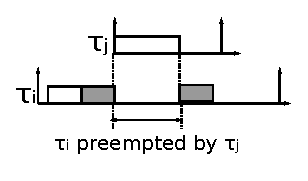
\includegraphics[scale=0.7]{figures/figure8}\caption{\label{fig8}Transactional retry due to release of higher priority
tasks}
\end{figure}
\end{comment}
\end{proof}

\begin{clm}\label{rcm rlease conflict}
Under RCM and G-RMA/LCM, the total retry cost suffered by all transactions in any $\tau_i^x$ during an interval $L\le T_i$ is upper bounded by:
\begin{equation}
RC_{to}(L)=RC(L)+RC_{re}(L)
\label{total rc rcm eq}
\end{equation}
%
where $RC(L)$ and $RC_{re}(L)$ are defined in Claim~\ref{ecm rlease conflict}. $RC(L)$ is calculated by (16) in~\cite{stmconcurrencycontrol:emsoft11} for RCM, and (8) in~\cite{lcmdac2012} for G-RMA/LCM. $RC_{re}(L)$ is calculated by:
\begin{equation}
RC_{re}(L)=\sum_{\forall \tau_j \in \zeta_i^*}\left(\left\lceil\frac{L}{T_j}\right\rceil s_{i_{max}}\right)\label{eq21}
\end{equation}
%
where $\zeta_i^*=\{\tau_j:p_j > p_i \}$.
\end{clm}
\begin{proof}
The proof is the same as that for Claim~\ref{ecm rlease conflict}, except that G-RMA uses static priority. Thus, the carried-out jobs will be considered in the  interference with $\tau_i^x$. The carried-in jobs are still not considered because they are released before $r_i^x$. Claim follows.
\end{proof}
\begin{clm}\label{lock free release}
Consider lock-free synchronization. Let $r_{i_{max}}$ be the maximum execution cost of a single iteration of any retry loop of $\tau_i$. $RC_{re}$ under G-EDF  with lock-free synchronization is calculated by~(\ref{eq6}), where $s_{i_{max}}$ is replaced by $r_{i_{max}}$. $RC_{re}$ under G-RMA with lock-free synchronization is calculated by~(\ref{eq21}), where $s_{i_{max}}$ is replaced by $r_{i_{max}}$.
\end{clm}
%
\begin{proof}
The interference pattern of higher priority jobs to lower priority jobs is the same in ECM, G-EDF/LCM, and G-EDF with lock-free. The pattern is also the same in RCM, G-RMA/LCM, and G-RMA with lock-free. 
%Claim follows.
\end{proof}


\subsection{PNF versus ECM\label{pnf vs ecm sec}}

\begin{clm}\label{PNF ecf comaprison clm}
In the absence of transitive retry, PNF/G-EDF's schedulability is better or equal to ECM's when conflicting atomic sections have equal lengths.
\end{clm}
\begin{proof}
Substitue $RC_{A}(T_{i})$ and $RC_{B}(T_{i})$ in (\ref{utilization comparison})
with (\ref{rc-PNF}) and (\ref{total rc ecm eq}), respectively. Let $\theta_{i}^{ex}=\theta_{i}+\theta_{i}^{*}$, where $\theta_{i}^{*}$
is the set of objects not accessed directly by $\tau_{i}$ but can
cause transactions in $\tau_{i}$ to retry due to transitive retry.
Let $\gamma_{i}^{ex}=\gamma_{i}+\gamma_{i}^{*}$, where $\gamma_{i}^{*}$
is the set of tasks that access objects in $\theta_{i}^{*}$.
Let:
%
\begin{comment}
\begin{eqnarray*}
g(\tau_{i}) & = & \left(\sum_{\forall\tau_{j}\in\gamma_{i}^{*}}\sum_{\theta\in\theta_{i}^{*}}\left(\left\lceil \frac{T_{i}}{T_{j}}\right\rceil \sum_{\forall\bar{s_{j}^{k}(\theta)}}len\left(\bar{s_{j}^{k}(\theta)}\\
& + & s_{max}(\theta)\right)\right)\right) + RC_{re}(T_{i})
\end{eqnarray*}
\end{comment}
\begin{eqnarray*}
g(\tau_{i}) & = & \Bigg(\sum_{\forall\tau_{j}\in\gamma_{i}^{*}}\sum_{\theta\in\theta_{i}^{*}}\Bigg(\left\lceil \frac{T_{i}}{T_{j}}\right\rceil \sum_{\forall\bar{s_{j}^{k}(\theta)}}len\Big(\bar{s_{j}^{k}(\theta)}\\
 & + & s_{max}(\theta)\Big)\Bigg)\Bigg)+RC_{re}(T_{i})
\end{eqnarray*}
%
where $RC_{re}$ is given by~(\ref{eq6}). $g(\tau_i)$ includes effect of transitive retry. Let:
%
\begin{equation*}
\eta_{1}(\tau_{i})=\sum_{\forall\tau_{j}\in\gamma_{i}}\sum_{\forall\theta\in\theta_{i}}\left(\sum_{\bar{\forall s_{j}^{k}(\theta)}}len\left(\bar{s_{j}^{k}(\theta)}\right)\right)
\end{equation*}
%
\begin{equation*}
\eta_{2}(\tau_{i})=\sum_{\forall\tau_{j}\in\gamma_{i}}\sum_{\forall\theta\in\theta_{i}}\left(\left\lceil \frac{T_{i}}{T_{j}}\right\rceil \sum_{\forall\bar{s_{j}^{k}(\theta)}}len\left(s_{max}^{j}(\theta)\right)\right)
\end{equation*}
%
%and
%
\begin{equation*}
\eta_{3}(\tau_{i})=\sum_{\forall\tau_{j}\in\gamma_{i}}\sum_{\forall\theta\in\theta_{i}}\left(\left\lceil \frac{T_{i}}{T_{j}}\right\rceil \sum_{\bar{\forall s_{j}^{k}(\theta)}}len\left(\bar{s_{j}^{k}(\theta)}\right)\right)
\end{equation*}
%
By substitution of $g(\tau_{i})$, $\eta_1(\tau_i)$, and $\eta_2(\tau_i)$, and subtraction of $\sum_{\forall \tau_i} \frac{\eta_3(\tau_i)}{T_i}$ from both sides of (\ref{utilization comparison}), we get: 
\begin{equation}
\sum_{\forall \tau_i} \frac{\eta_1(\tau_i)}{T_i} \le \sum_{\forall \tau_i} \frac{\eta_2(\tau_i)+g(\tau_i)}{T_i}
\label{PNF ecm comparison 2}
\end{equation}
Assume that $g(\tau_{i})_{\forall\tau_{i}}\rightarrow0$. From (\ref{PNF ecm comparison 2}), we note that by keeping
every $len(\bar{s_{j}^{k}(\theta)})\le len(s_{max}^{j}(\theta))$
for each $\tau_{i}$, $\tau_{j}\in\gamma_{i}$, and $\theta\in\theta_{i}$,  (\ref{PNF ecm comparison 2}) holds. 
%
Due to G-EDF's dynamic priority, $s_{max}^{j}(\theta)$
can belong to any task other than $\tau_{j}$. By keeping $len(\bar{s_j^k(\theta)})\le len(s_{max}^j(\theta))$, then~\ref{PNF ecm comparison 2} holds. By generalizing this condition to any $s_j^k(\theta)$ and $s_{max}^j(\theta)$, then~\ref{PNF ecm comparison 2} holds if all atomic sections in all tasks have equal lengths. Claim follows.
\end{proof}

\subsection{PNF versus RCM}\label{pnf vs rcm sec}

\begin{clm}\label{clm_pnf_rcm_comp}
In the absence of transitive retry, PNF/G-RMA's schedulability is better or equal to RCM's schedulability when a large number of tasks heavily conflict. PNF's schedulability is improved compared with RCM's, when atomic section length increases as priority increases. 
\end{clm}
\begin{proof}
Let $\theta_{i}^{ex}=\theta_{i}+\theta_{i}^{*}$ and $\gamma_{i}^{ex}=\gamma_{i}+\gamma_{i}^{*}$, as defined in the proof of Claim~\ref{PNF ecf comaprison clm}. Substitute $RC_{A}(T_{i})$ and $RC_{B}(T_{i})$ in (\ref{utilization comparison}) with (\ref{rc-PNF}) and (\ref{total rc rcm eq}), respectively. Let: 
% 
\begin{eqnarray*}
g(\tau_{i}) & =RC_{re}(T_{i})+\Bigg( & \sum_{\forall\tau_{j}\in(\gamma_{i}^{*}\cap\zeta_{i}^{*})}\sum_{\forall\theta\in\theta_{i}^{*}}\left(\left\lceil \frac{T_{i}}{T_{j}}\right\rceil +1\right)\times\\
 &  & \sum_{\forall\bar{s_{j}^{k}(\theta)}}len\left(\bar{s_{j}^{k}(\theta)}+s_{max}^{j}(\theta)\right)\Bigg)
\end{eqnarray*}
%
where $RC_{re}$ and $\zeta_i^*$ are defined by~(\ref{eq21}). $g(\tau_i)$ includes effect of transitive retry. 
Let $\gamma_{i}=\zeta_{i}^{*}\cup\bar{\zeta_{i}}$, where $\bar{\zeta_{i}}=\left\{ \tau_{j}:\left(\tau_{j}\ne\tau_{i}\right)\wedge\left(p_{j}<p_{i}\right)\right\} $,
thus $\zeta_{i}^{*}\cap\bar{\zeta_{i}}=\phi$.

Let:
%
\begin{equation*}
\eta_{1}(\tau_{i})=\sum_{\forall\tau_{j}\in(\gamma_{i}\cap\zeta_{i}^{*})}\sum_{\forall\theta\in\theta_{i}}\left(\left(\left\lceil \frac{T_{i}}{T_{j}}\right\rceil +1\right)\sum_{\bar{\forall s_{j}^{k}(\theta)}}len\left(\bar{s_{j}^{k}(\theta)}\right)\right)
\end{equation*}
%
\begin{equation*}
\eta_{2}(\tau_{i})=\sum_{\forall\tau_{j}\in(\gamma_{i}\cap\bar{\zeta_{i}})}\sum_{\forall\theta\in\theta_{i}}\left(\left(\left\lceil \frac{T_{i}}{T_{j}}\right\rceil +1\right)\sum_{\bar{\forall s_{j}^{k}(\theta)}}len\left(\bar{s_{j}^{k}(\theta)}\right)\right)
\end{equation*}
%
%and
%
\begin{eqnarray*}
\eta_{3}(\tau_{i}) & = & \sum_{\forall\tau_{j}\in(\gamma_{i}\cap\zeta_{i}^{*})}\sum_{\forall\theta\in\theta_{i}}\Bigg(\left(\left\lceil \frac{T_{i}}{T_{j}}\right\rceil +1\right)\times\\
 &  & \sum_{\forall\bar{s_{j}^{k}(\theta)}}len\left(\bar{s_{j}^{k}(\theta)}+s_{max}^{j}(\theta)\right)\Bigg)
\end{eqnarray*}
%
By substitution of $g(\tau_i)$, $\eta_1(\tau_i)$, $\eta_2(\tau_i)$, and $\eta_3(\tau_i)$ in (\ref{utilization comparison}):
%
\begin{equation}
\sum_{\forall\tau_{i}}\frac{\eta_{1}(\tau_{i})+\eta_{2}(\tau_{i})}{T_{i}}\le\sum_{\forall\tau_{i}}\frac{\eta_{3}(\tau_{i})+g(\tau_{i})}{T_{i}}
\label{PNF rcm comparison 3}
\end{equation}
%
When tasks with deadlines equal to periods are scheduled with G-RMA, $T_{j}>T_{i}$ if $p_{j}<p_{i}$. So, for each $\tau_{j}\in\bar{\zeta_{i}}$, $\left\lceil \frac{T_{i}}{T_{j}}\right\rceil =1$. Then:
%
\begin{equation}
\eta_{2}(\tau_{i})=2\sum_{\forall\tau_{j}\in(\gamma_{i}\cap\bar{\zeta_{i}})}\sum_{\forall\theta\in\theta_{i}}\sum_{\bar{\forall s_{j}^{k}(\theta)}}len\left(\bar{s_{j}^{k}(\theta)}\right)
\label{PNF rcm comparison 5}
\end{equation}
%
Let:
%
\begin{equation*}
\eta_{4}(\tau_{i})=\sum_{\forall\tau_{j}\in(\gamma_{i}\cap\zeta_{i}^{*})}\sum_{\forall\theta\in\theta_{i}}\left(\left\lceil \frac{T_{i}}{T_{j}}\right\rceil +1\right)\sum_{\forall\bar{s_{j}^{k}(\theta)}}len\left(s_{max}^{j}(\theta)\right)
\end{equation*}
%
By substitution of~(\ref{PNF rcm comparison 5}) and subtraction of $\sum_{\forall \tau_i} \frac{\eta_1 (\tau_i)}{T_i}$ from both sides of~(\ref{PNF rcm comparison 3}), we get:
%
\begin{equation}
2\sum_{\forall\tau_{i}}\frac{\eta_{2}(\tau_{i})}{T_{i}}\le\sum_{\forall\tau_{i}}\frac{\eta_{4}(\tau_{i})+g(\tau_{i})}{T_{i}}
\label{PNF rcm comparison 4}
\end{equation}
%
Assume that $g(\tau_{i})_{\forall\tau_{i}}\rightarrow0$. From (\ref{PNF rcm comparison 4}), we note that when higher priority jobs increasingly conflict with lower priority jobs, (\ref{PNF rcm comparison 4}) tends to hold. (\ref{PNF rcm comparison 4}) also tends to hold if $len(\bar{s_{max}^j(\theta)})$ in the right hand side of (\ref{PNF rcm comparison 4}) is larger than $len(\bar{s_j^k(\theta)})$ in the left hand side of (\ref{PNF rcm comparison 4}), which means atomic section length increases as priority increases. Claim follows.
\end{proof}

\subsection{PNF versus G-EDF/LCM}

\begin{clm}\label{sub:pnf_lcm_edf_comp}
In the absence of transitive retry, PNF/EDF's schedulability is equal or better than G-EDF/LCM's if the conflicting atomic section lengths are approximately equal and all $\alpha$ terms approach 1.

\end{clm}
\begin{proof}
Assume that $\eta_{1}(\tau_i)$ and $\eta_{3}(\tau_i)$ are the same as that defined in the proof
of Claim~\ref{PNF ecf comaprison clm}. Let:
\begin{eqnarray*}
g(\tau_{i}) & = & \Bigg(\sum_{\forall\tau_{j}\in\gamma_{i}^{*}}\sum_{\theta\in\theta_{i}^{*}}\Bigg(\left\lceil \frac{T_{i}}{T_{j}}\right\rceil \sum_{\forall\bar{s_{j}^{k}(\theta)}}len\Big(\bar{s_{j}^{k}(\theta)}\\
 & + & \alpha_{max}^{ji}s_{max}(\theta)\Big)\Bigg)\Bigg)+RC_{re}(T_{i})
\end{eqnarray*}
\[
\eta_{2}(\tau_{i})=\sum_{\forall\tau_{j}\in\gamma_{i}}\sum_{\forall\theta\in\theta_{i}}\left(\left\lceil \frac{T_{i}}{T_{j}}\right\rceil \sum_{\forall\bar{s_{j}^{k}(\theta)}}len\left(\alpha_{max}^{jl}s_{max}^{j}(\theta)\right)\right)
\]
where $\alpha_{max}^{jl}$ is defined in~(\ref{eq78}). Following the same steps in the proof of Claim~\ref{PNF ecf comaprison clm}, we get:
\begin{equation}
\sum_{\forall\tau_{i}}\frac{\eta_{1}(\tau_{i})}{T_{i}}\le\sum_{\forall\tau_{i}}\frac{\eta_{2}(\tau_{i})+g(\tau_{i})}{T_{i}}\label{eq:pnf_lcm_edf_comp}
\end{equation}
Assume that $g(\tau_{i})_{\forall\tau_{i}}\rightarrow0$. Thus, we ignore the effect of transitive retry and retry cost due to the release of higher priority jobs. Let $len(\bar{s_{j}^{k}(\theta)})=s_{max}^{j}(\theta)=s$,
and $\alpha_{max}^{jl}=\alpha_{max}^{iy}=1$ in (\ref{eq:pnf_lcm_edf_comp}). Then, PNF/EDF's schedulability equals LCM/EDF's schedulability if
$\left\lceil \frac{T_{i}}{T_{j}}\right\rceil =1,\,\forall\tau_{i},\tau_{j}$
(which means equal periods for all tasks). If $\left\lceil \frac{T_{i}}{T_{j}}\right\rceil >1,\,\forall\tau_{i},\tau_{j}$,
PNF/EDF's schedulability is better than LCM/EDF's. PNF/EDF's schedulability  becomes more better than LCM/EDF's schedulability if $g(\tau_{i})$
is not zero. Claim follows.
\end{proof}

%\begin{comment}
\subsection{PNF versus G-RMA/LCM}

\begin{clm}\label{sub:pnf_lcm_rma_comp}
%
In the absence of transitive retry, PNF's schedulability is equal or better than G-RMA/LCM's if: 1) lower priority tasks suffer increasing number of conflicts from higher priority tasks, 2) the lengths of the atomic sections increase as task priorities increase, and 3) $\alpha$ terms increase.
%
\end{clm}
\begin{proof}
Assume that $g(\tau_{i})$, $\eta_{1}(\tau_{i})$, and $\eta_{2}(\tau_{i})$ are the same as in the proof of Claim~\ref{clm_pnf_rcm_comp}. Let:
\begin{eqnarray*}
\eta_{3}(\tau_{i}) & = & \sum_{\forall\tau_{j}\in(\gamma_{i}\cap\zeta_{i}^{*})}\sum_{\forall\theta\in\theta_{i}}\Bigg(\left(\left\lceil \frac{T_{i}}{T_{j}}\right\rceil +1\right)\times\\
 &  & \sum_{\forall\bar{s_{j}^{k}(\theta)}}len\left(\bar{s_{j}^{k}(\theta)}+\alpha_{max}^{jl}s_{max}^{j}(\theta)\right)\Bigg)
\end{eqnarray*}
%and
\begin{eqnarray*}
\eta_{4}(\tau_{i}) & = & \sum_{\forall\tau_{j}\in(\gamma_{i}\cap\zeta_{i}^{*})}\sum_{\forall\theta\in\theta_{i}}\Bigg(\left(\left\lceil \frac{T_{i}}{T_{j}}\right\rceil +1\right)\\
 & \times & \sum_{\forall\bar{s_{j}^{k}(\theta)}}len\left(\alpha_{max}^{jl}s_{max}^{j}(\theta)\right)\Bigg)
\end{eqnarray*}
Following the steps of Claim~\ref{clm_pnf_rcm_comp}'s proof, 
$\therefore$(\ref{utilization comparison}) becomes:
\begin{equation}
2\sum_{\forall\tau_{i}}\frac{\eta_{2}(\tau_{i})}{T_{i}}\le\sum_{\forall\tau_{i}}\frac{\eta_{4}(\tau_{i})+g(\tau_{i})}{T_{i}}\label{pnf-lcm-rma-comp-2}
\end{equation}
Assume that the effect of transitive retry and retry cost due
to the release of higher priority jobs is negligible ($g(\tau_{i})\rightarrow0$). (\ref{pnf-lcm-rma-comp-2})
holds if: 1) the contention from higher priority jobs to lower priority
jobs increases because of the $\left\lceil \frac{T_{i}}{T_{j}}\right\rceil +1$
term in the right hand side of (\ref{pnf-lcm-rma-comp-2}); 2) $\alpha$ terms
approach 1; and 3) the lengths of the atomic sections increase as priority
increases. 
%
This makes $len(s_{max}^{j}(\theta))$ in (\ref{pnf-lcm-rma-comp-2})'s right 
side to be greater than $len(\bar{s_{j}^{k}(\theta)})$ in (\ref{pnf-lcm-rma-comp-2})'s left  side.
Claim follows.
\end{proof}
%\end{comment}

\subsection{PNF versus Lock-free Synchronization\label{pnf vs lock free sec}}

Lock-free synchronization~\cite{key-5,stmconcurrencycontrol:emsoft11} accesses only one object. Thus, the number of accessed objects per transaction in PNF is limited to one. This allows us to compare the schedulability of PNF with the lock-free algorithm. 

$RC_{B}(T_{i})$ in (\ref{utilization comparison}) is replaced with:
%
\begin{equation}
\sum_{\forall\tau_{j}\in\gamma_{i}}\Bigg(\left(\left\lceil \frac{T_{i}}{T_{j}}\right\rceil +1\right)\beta_{i,j}r_{max}\Bigg)+RC_{re}(T_{i})
\label{lock-free rc}
\end{equation}
%
where $\beta_{i,j}$ is the number of retry loops of $\tau_{j}$ that access the same object as accessed by some retry loop of $\tau_{i}$~\cite{key-5}. $r_{max}$ is the maximum execution cost of a single iteration of any retry loop of any task~\cite{key-5}. $RC_{re}(T_i)$ is defined in Claim~\ref{lock free release}. Lock-free synchronization does not depend on priorities  of tasks. Thus,~(\ref{lock-free rc}) applies for both G-EDF and G-RMA systems.


%%
\begin{clm}\label{PNF lock-free comparison}
Let $r_{max}$ be the maximum execution cost of a single iteration of any retry loop of any task~\cite{key-5}. Let $s_{max}$ be the maximum transaction length in all tasks. Assume that each transaction under PNF accesses only one object for once. The schedulability of PNF with either G-EDF or G-RMA scheduler is better or equal to the schedulability of lock-free
synchronization if $s_{max}/r_{max}\le 1$.
\end{clm}
\begin{proof}
The assumption in Claim~\ref{PNF lock-free comparison} is made to enable a comparison between PNF and lock-free. Let $RC_{A}(T_{i})$ in (\ref{utilization comparison}) be replaced
with (\ref{rc-PNF}) and $RC_{B}(T_{i})$ be replaced with (\ref{lock-free rc}).
To simplify comparison, (\ref{rc-PNF}) is upper bounded by:
%
\begin{equation*}
RC(T_{i})=\sum_{\tau_{j}\in\gamma_{i}}\left(\left(\left\lceil \frac{T_{i}}{T_{j}}\right\rceil +1\right)\beta_{i,j}^* s_{max}\right)
\end{equation*}
%
where $\beta_{i,j}^*$ is the number of times transactions in $\tau_j$ accesses shared objects with $
\tau_i$. Thus, $\beta_{i,j}^* = \beta_{i,j}$, and (\ref{utilization comparison}) will be:
\begin{eqnarray}
\sum_{\forall\tau_{i}}\frac{\sum_{\tau_{j}\in\gamma_{i}}\left(\left(\left\lceil \frac{T_{i}}{T_{j}}\right\rceil +1\right)\beta_{i,j}s_{max}\right)}{T_{i}} & \le\nonumber \\
\sum_{\forall\tau_{i}}\frac{\sum_{\forall\tau_{j}\in\gamma_{i}}\left(\left\lceil \frac{T_{i}}{T_{j}}\right\rceil +1\right)\beta_{i,j}r_{max}+RC_{re}(\tau_i)}{T_{i}}\label{eq:PNF lock-free comparison}
\end{eqnarray}
From (\ref{eq:PNF lock-free comparison}), we note that if $s_{max}\le r_{max}$,
then (\ref{eq:PNF lock-free comparison}) holds. 
%Claim follows.
\end{proof}

%%%
\section{Experimental Evaluation}\label{exp_eval}

%Having established PNF's retry and response time bounds, and the conditions under which it outperforms ECM, RCM, LCM, and lock-free synchronization, 
We now would like to understand how PNF's retry cost compares with competitors in practice (i.e., on average). Since this can only be understood experimentally, we implement PNF and the competitors and conduct experiments. 

%\subsection{Experimental Setup}

We used the ChronOS real-time Linux kernel~\cite{dellinger2011chronos}
and the RSTM library~\cite{marathe2006lowering} in our implementation. We implemented G-EDF and G-RMA schedulers in ChronOS, and modified RSTM to include implementations of ECM, RCM, LCM, and PNF. For the retry-loop lock-free synchronization, we used a loop that reads an object and attempts to write to it  using a CAS  instruction. The task retries until the CAS succeeds. We used an 8 core, 2GHz AMD Opteron platform. The average time taken for one write operation by RSTM on any core is 0.0129653375$\mu s$, and the average time taken by one CAS-loop operation on any core is 0.0292546250 $\mu s$.

We used four task sets consisting of 4, 5, 8, and 20 periodic tasks. Each task runs in its own thread and has a set of atomic sections. Atomic section properties are probabilistically controlled using three parameters: the maximum and minimum lengths of any atomic section within a task, and the total length of atomic sections within any task. Since lock-free synchronization cannot handle more than one object per atomic section, we first compare PNF's retry cost with that of lock-free (and other CMs) for one object per transaction. We then compare PNF's retry cost with that of other CMs for multiple objects per transaction.

\begin{figure}
\centering
\subfigure[ECM, RCM, LCM, PNF, Lock-Free]{
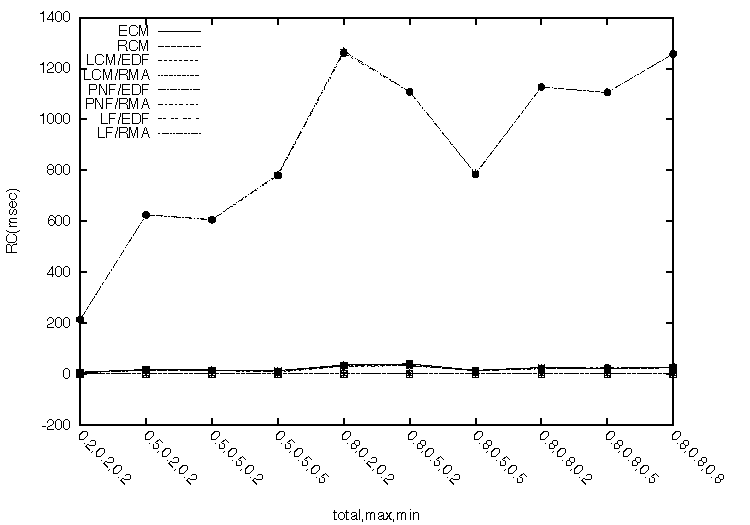
\includegraphics[scale=0.6]
{figures/Abr_dur_5t_1obj_1wr}
\label{fig:pnf_results_1_obj_all}
}
%~
\subfigure[ECM, RCM, LCM, PNF]{
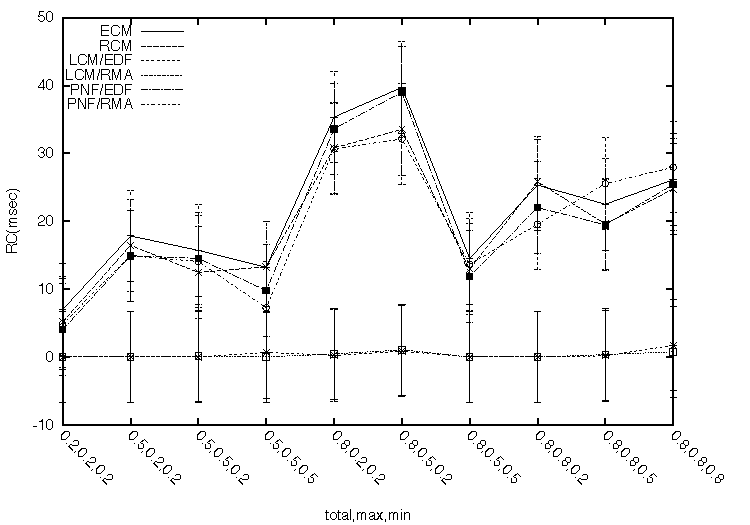
\includegraphics[scale=0.6]
{figures/Abr_dur_5t_1obj_1wr_without_lf}
\label{fig:pnf_results_1_obj_without_lock_free}
}
\caption{Avg. retry cost (one object/transaction).}
\label{fig:pnf_results_uniobject}
\end{figure}

Figures~\ref{fig:pnf_results_uniobject} and~\ref{fig-RC-pnf-4t} show the average retry cost for the 5 task and 4 task case, respectively, under 1 and 5 shared objects, respectively. 
On the x-axis of the figures, we record 3 parameters $x$, $y$, and $z$. $x$ is the ratio of the total length of all atomic sections of a task to the task WCET. $y$ is the ratio of the maximum length of any atomic section of a task to the task WCET. $z$ is the ratio of the minimum length of any atomic section of a task to the task WCET. Confidence level of all data points is 0.95.
 
While Figure~\ref{fig:pnf_results_1_obj_all} includes all methods, Figure~\ref{fig:pnf_results_1_obj_without_lock_free} excludes lock-free. From these figures, we observe that lock-free has the largest retry cost, as it provides no conflict resolution. LCM is better than the others. PNF's retry cost closely approximates ECM's and RCMs, as there is no transitive retry. From Figure~\ref{fig-RC-pnf-4t}, we observe that PNF has shorter or comparable retry cost than ECM, RCM, and LCM.

 Similar trends were observed for the other task sets.
 %; those are omitted here for brevity and due to space limitations. 


\begin{comment}
In Figure~\ref{fig-RC-pnf-20t}, retry costs are close. This happens because each task's execution time is small relative to the task's period. Consequently, atomic sections have small length and are highly unlikely to be triggered at the same time. Thus, contention, as well as, retry costs are low.
\end{comment}


\begin{figure}
\centering
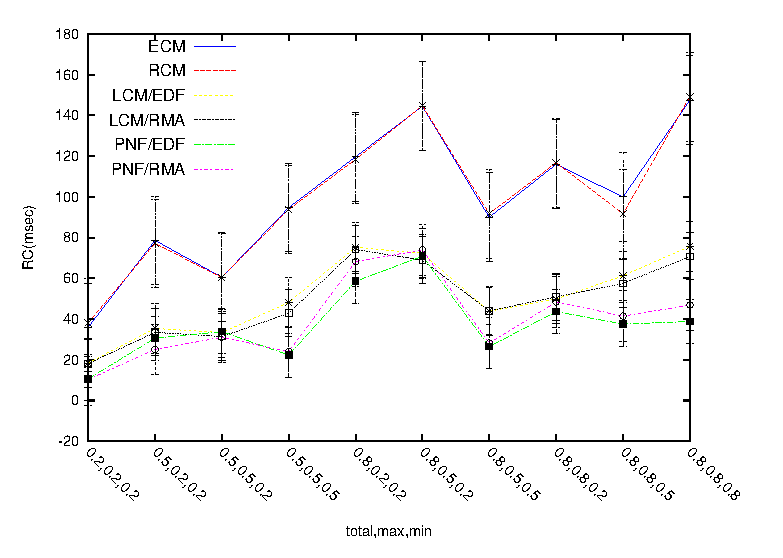
\includegraphics[scale=0.6]{figures/Abr_dur_4t_5obj_1wr}
\caption{Avg. retry cost (5 shared objects, 4 tasks).}
\label{fig-RC-pnf-4t}
\end{figure}

\begin{comment}
\begin{figure}
\centering
\subfigure[Task set 1 (4 tasks)]{
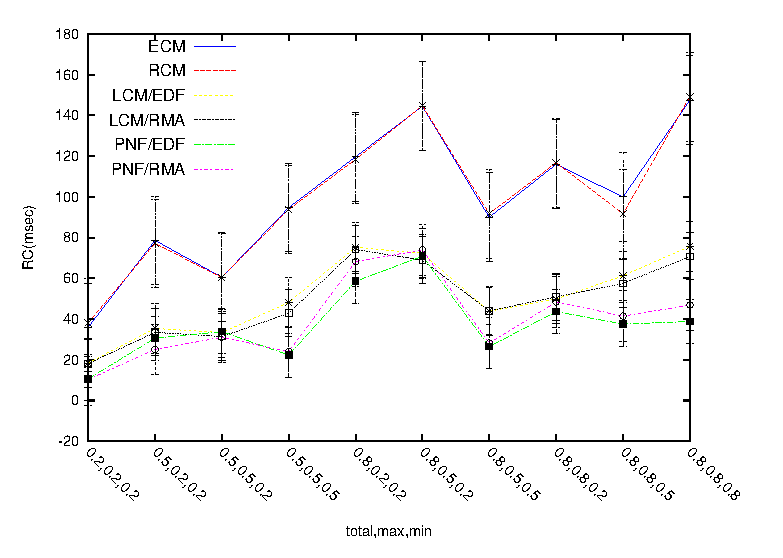
\includegraphics[scale=0.6]
{figures/Abr_dur_4t_5obj_1wr}
\label{fig-RC-pnf-4t}
}
~
\subfigure[Task set 2 (8 tasks)]{
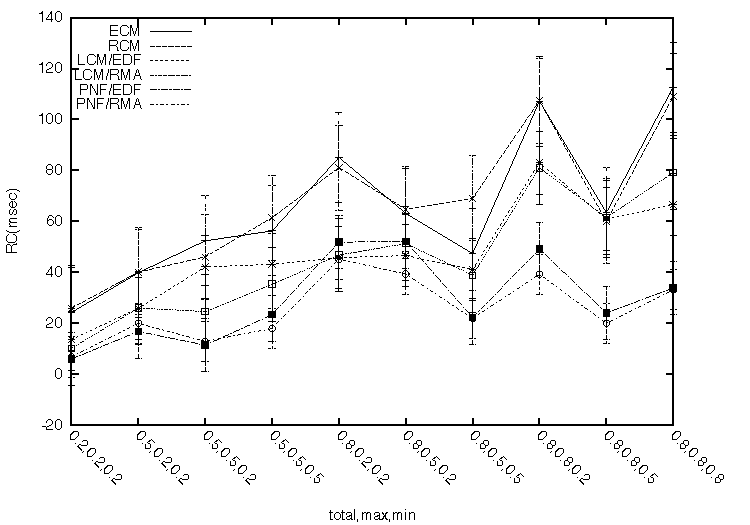
\includegraphics[scale=0.6]
{figures/Abr_dur_8t_9obj_1wr}
\label{fig-RC-pnf-8t}
}
~
\subfigure[Task set 3 (20 tasks)]{
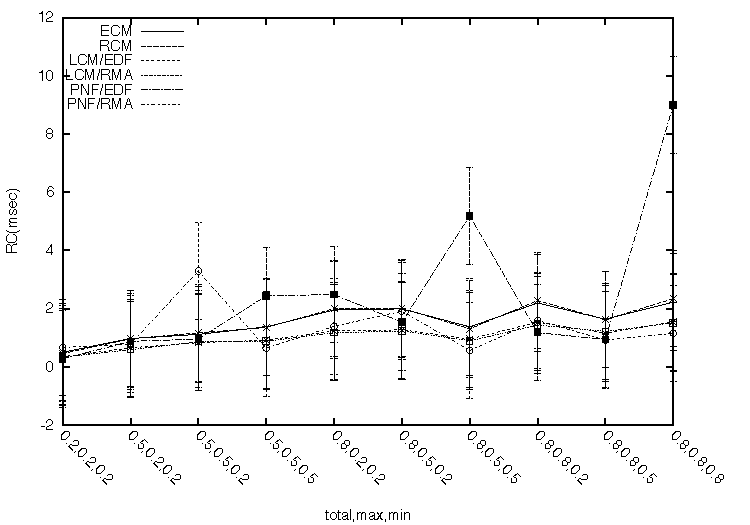
\includegraphics[scale=0.5]{figures/Abr_dur_20t_21obj_1wr}
\label{fig-RC-pnf-20t}
}
\caption{Average retry cost under multiple objects per transaction.}
\label{fig:pnf_results_multiobject}
\end{figure}
\end{comment}


\section{Conclusions}\label{conclusion}

Transitive retry increases transactional retry cost under ECM, RCM, and LCM. PNF avoids transitive retry by avoiding   transactional preemptions. PNF reduces the priority of aborted transactions to enable other tasks to execute, increasing processor usage. Executing transactions are not preempted due to the release of higher priority jobs. On the negative side of PNF, higher priority jobs can be blocked by executing transactions of lower priority jobs. 

EDF/PNF's schedulability is equal or better than ECM's when atomic section lengths are almost equal. RMA/PNF's schedulability is equal or better than RCM's when lower priority jobs suffer greater conflicts from higher priority ones. Similar conditions hold for the schedulability comparison between PNF and LCM, in addition to the increase of $\alpha$ terms to 1. This is logical as LCM with G-EDF (G-RMA) defaults to ECM (RCM) with $\alpha\rightarrow 1$. For PNF's schedulability to be equal or better than lock-free, the upper bound on $s_{max}/r_{max}$ must be 1, instead of 0.5 under ECM and RCM. 

%An interesting future direction is how to combine PNF and LCM, which defaults to PNF for high  transitive retry cases, and LCM otherwise, reducing retry costs in all cases.

%%BR: DONE. 1:44AM, April 12, 2012. 

\bibliographystyle{abbrv}
\small{\bibliography{global_bibliography}}

\end{document}
